\documentclass[1p]{elsarticle_modified}
%\bibliographystyle{elsarticle-num}

%\usepackage[colorlinks]{hyperref}
%\usepackage{abbrmath_seonhwa} %\Abb, \Ascr, \Acal ,\Abf, \Afrak
\usepackage{amsfonts}
\usepackage{amssymb}
\usepackage{amsmath}
\usepackage{amsthm}
\usepackage{scalefnt}
\usepackage{amsbsy}
\usepackage{kotex}
\usepackage{caption}
\usepackage{subfig}
\usepackage{color}
\usepackage{graphicx}
\usepackage{xcolor} %% white, black, red, green, blue, cyan, magenta, yellow
\usepackage{float}
\usepackage{setspace}
\usepackage{hyperref}

\usepackage{tikz}
\usetikzlibrary{arrows}

\usepackage{multirow}
\usepackage{array} % fixed length table
\usepackage{hhline}

%%%%%%%%%%%%%%%%%%%%%
\makeatletter
\renewcommand*\env@matrix[1][\arraystretch]{%
	\edef\arraystretch{#1}%
	\hskip -\arraycolsep
	\let\@ifnextchar\new@ifnextchar
	\array{*\c@MaxMatrixCols c}}
\makeatother %https://tex.stackexchange.com/questions/14071/how-can-i-increase-the-line-spacing-in-a-matrix
%%%%%%%%%%%%%%%

\usepackage[normalem]{ulem}

\newcommand{\msout}[1]{\ifmmode\text{\sout{\ensuremath{#1}}}\else\sout{#1}\fi}
%SOURCE: \msout is \stkout macro in https://tex.stackexchange.com/questions/20609/strikeout-in-math-mode

\newcommand{\cancel}[1]{
	\ifmmode
	{\color{red}\msout{#1}}
	\else
	{\color{red}\sout{#1}}
	\fi
}

\newcommand{\add}[1]{
	{\color{blue}\uwave{#1}}
}

\newcommand{\replace}[2]{
	\ifmmode
	{\color{red}\msout{#1}}{\color{blue}\uwave{#2}}
	\else
	{\color{red}\sout{#1}}{\color{blue}\uwave{#2}}
	\fi
}

\newcommand{\Sol}{\mathcal{S}} %segment
\newcommand{\D}{D} %diagram
\newcommand{\A}{\mathcal{A}} %arc


%%%%%%%%%%%%%%%%%%%%%%%%%%%%%5 test

\def\sl{\operatorname{\textup{SL}}(2,\Cbb)}
\def\psl{\operatorname{\textup{PSL}}(2,\Cbb)}
\def\quan{\mkern 1mu \triangleright \mkern 1mu}

\theoremstyle{definition}
\newtheorem{thm}{Theorem}[section]
\newtheorem{prop}[thm]{Proposition}
\newtheorem{lem}[thm]{Lemma}
\newtheorem{ques}[thm]{Question}
\newtheorem{cor}[thm]{Corollary}
\newtheorem{defn}[thm]{Definition}
\newtheorem{exam}[thm]{Example}
\newtheorem{rmk}[thm]{Remark}
\newtheorem{alg}[thm]{Algorithm}

\newcommand{\I}{\sqrt{-1}}
\begin{document}

%\begin{frontmatter}
%
%\title{Boundary parabolic representations of knots up to 8 crossings}
%
%%% Group authors per affiliation:
%\author{Yunhi Cho} 
%\address{Department of Mathematics, University of Seoul, Seoul, Korea}
%\ead{yhcho@uos.ac.kr}
%
%
%\author{Seonhwa Kim} %\fnref{s_kim}}
%\address{Center for Geometry and Physics, Institute for Basic Science, Pohang, 37673, Korea}
%\ead{ryeona17@ibs.re.kr}
%
%\author{Hyuk Kim}
%\address{Department of Mathematical Sciences, Seoul National University, Seoul 08826, Korea}
%\ead{hyukkim@snu.ac.kr}
%
%\author{Seokbeom Yoon}
%\address{Department of Mathematical Sciences, Seoul National University, Seoul, 08826,  Korea}
%\ead{sbyoon15@snu.ac.kr}
%
%\begin{abstract}
%We find all boundary parabolic representation of knots up to 8 crossings.
%
%\end{abstract}
%\begin{keyword}
%    \MSC[2010] 57M25 
%\end{keyword}
%
%\end{frontmatter}

%\linenumbers
%\tableofcontents
%
\newcommand\colored[1]{\textcolor{white}{\rule[-0.35ex]{0.8em}{1.4ex}}\kern-0.8em\color{red} #1}%
%\newcommand\colored[1]{\textcolor{white}{ #1}\kern-2.17ex	\textcolor{white}{ #1}\kern-1.81ex	\textcolor{white}{ #1}\kern-2.15ex\color{red}#1	}

{\Large $\underline{12n_{0754}~(K12n_{0754})}$}

\setlength{\tabcolsep}{10pt}
\renewcommand{\arraystretch}{1.6}
\vspace{1cm}\begin{tabular}{m{100pt}>{\centering\arraybackslash}m{274pt}}
\multirow{5}{120pt}{
	\centering
	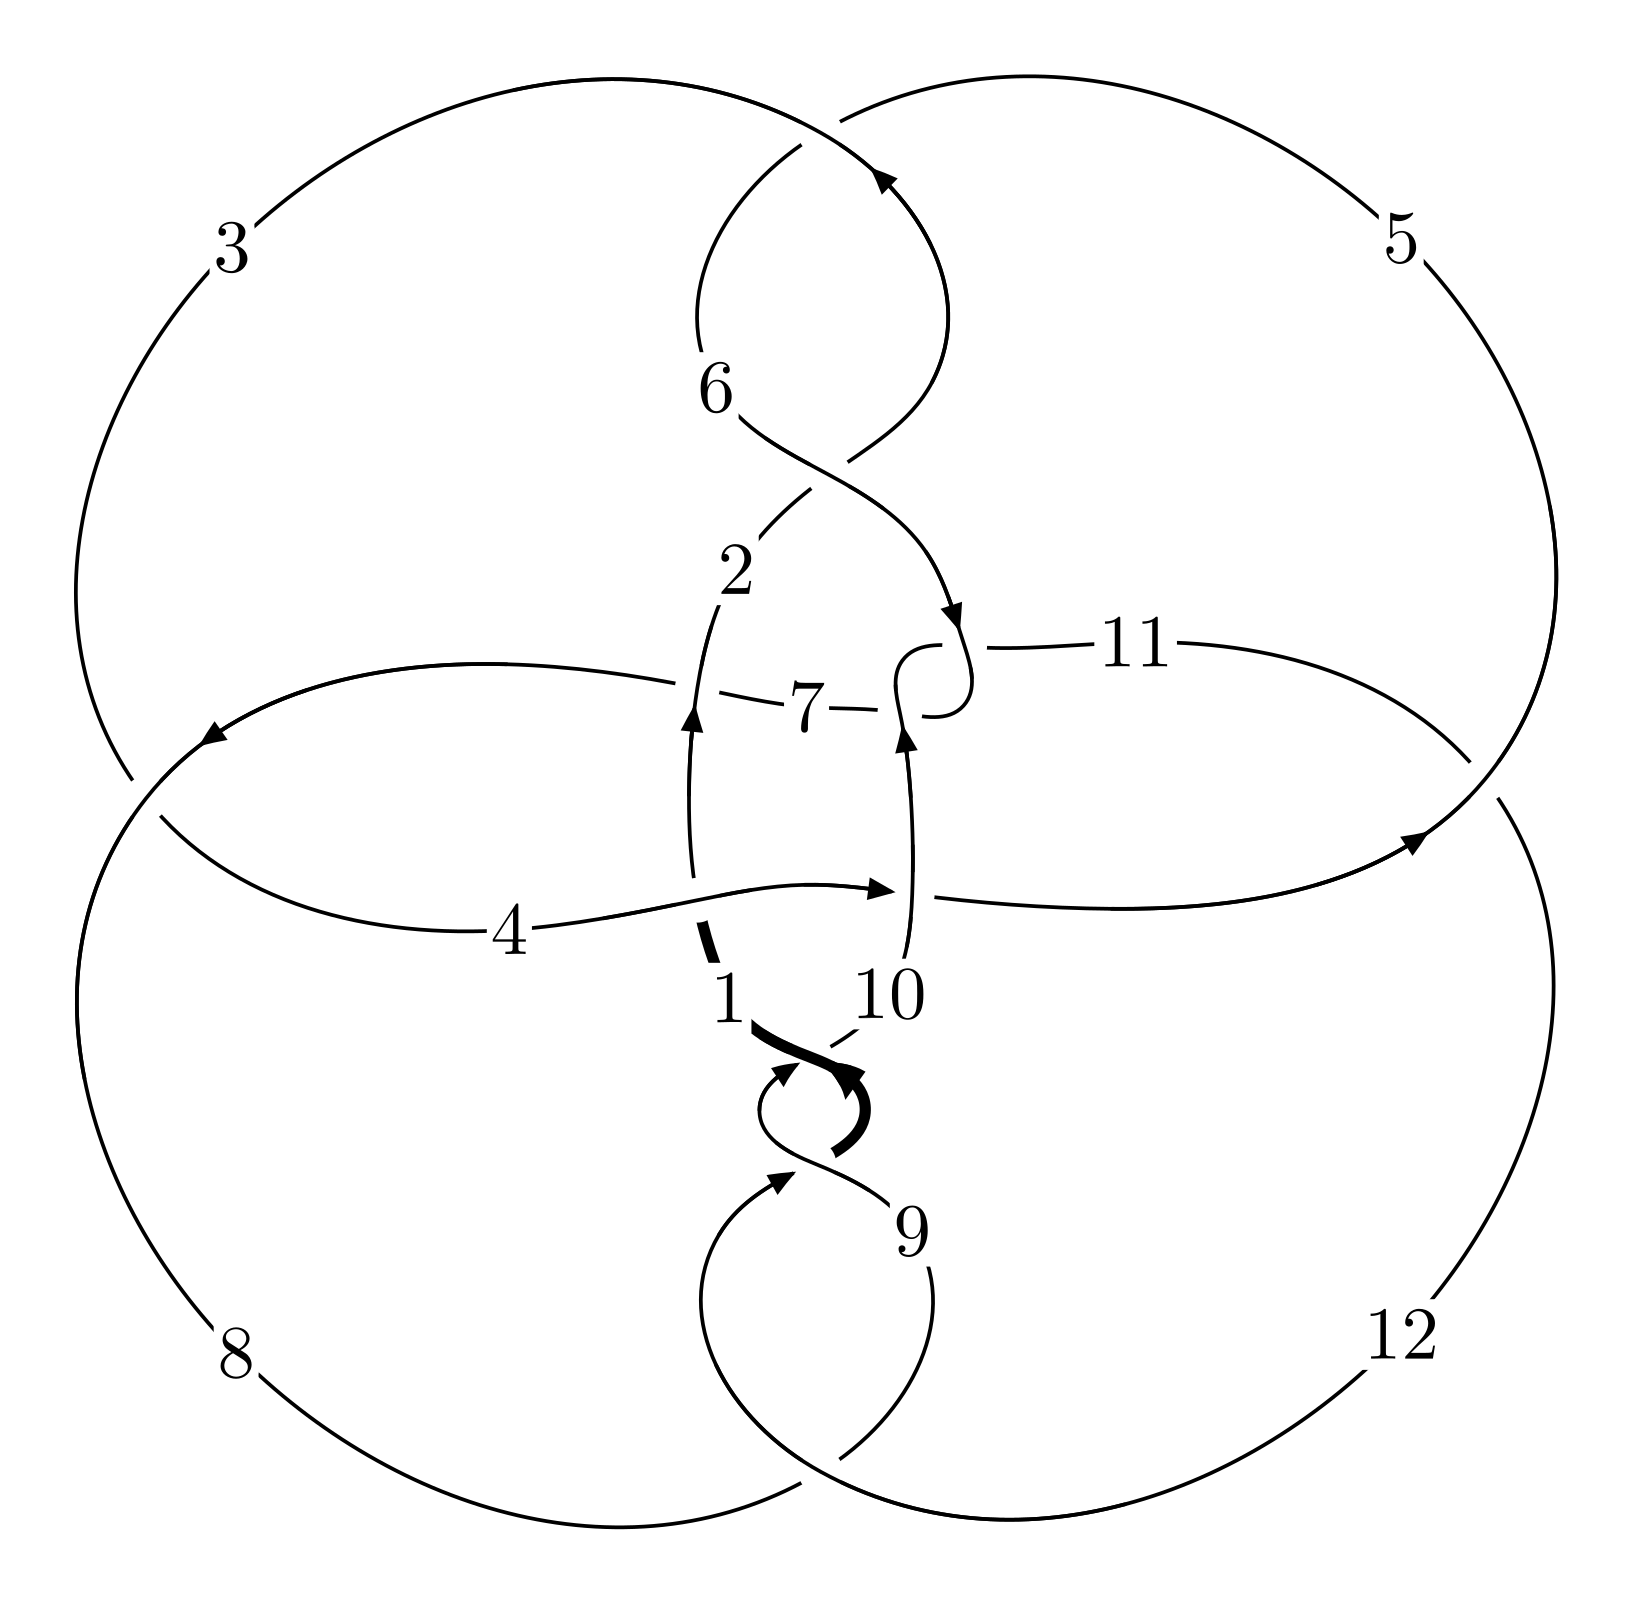
\includegraphics[width=112pt]{../../../GIT/diagram.site/Diagrams/png/2843_12n_0754.png}\\
\ \ \ A knot diagram\footnotemark}&
\allowdisplaybreaks
\textbf{Linearized knot diagam} \\
\cline{2-2}
 &
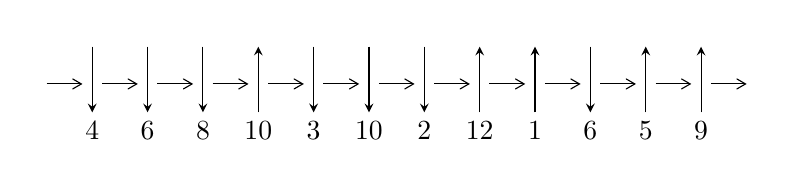
\begin{tikzpicture}[x=20pt, y=17pt]
	% nodes
	\node (C0) at (0, 0) {};
	\node (C1) at (1, 0) {};
	\node (C1U) at (1, +1) {};
	\node (C1D) at (1, -1) {4};

	\node (C2) at (2, 0) {};
	\node (C2U) at (2, +1) {};
	\node (C2D) at (2, -1) {6};

	\node (C3) at (3, 0) {};
	\node (C3U) at (3, +1) {};
	\node (C3D) at (3, -1) {8};

	\node (C4) at (4, 0) {};
	\node (C4U) at (4, +1) {};
	\node (C4D) at (4, -1) {10};

	\node (C5) at (5, 0) {};
	\node (C5U) at (5, +1) {};
	\node (C5D) at (5, -1) {3};

	\node (C6) at (6, 0) {};
	\node (C6U) at (6, +1) {};
	\node (C6D) at (6, -1) {10};

	\node (C7) at (7, 0) {};
	\node (C7U) at (7, +1) {};
	\node (C7D) at (7, -1) {2};

	\node (C8) at (8, 0) {};
	\node (C8U) at (8, +1) {};
	\node (C8D) at (8, -1) {12};

	\node (C9) at (9, 0) {};
	\node (C9U) at (9, +1) {};
	\node (C9D) at (9, -1) {1};

	\node (C10) at (10, 0) {};
	\node (C10U) at (10, +1) {};
	\node (C10D) at (10, -1) {6};

	\node (C11) at (11, 0) {};
	\node (C11U) at (11, +1) {};
	\node (C11D) at (11, -1) {5};

	\node (C12) at (12, 0) {};
	\node (C12U) at (12, +1) {};
	\node (C12D) at (12, -1) {9};
	\node (C13) at (13, 0) {};

	% arrows
	\draw[->,>={angle 60}]
	(C0) edge (C1) (C1) edge (C2) (C2) edge (C3) (C3) edge (C4) (C4) edge (C5) (C5) edge (C6) (C6) edge (C7) (C7) edge (C8) (C8) edge (C9) (C9) edge (C10) (C10) edge (C11) (C11) edge (C12) (C12) edge (C13) ;	\draw[->,>=stealth]
	(C1U) edge (C1D) (C2U) edge (C2D) (C3U) edge (C3D) (C4D) edge (C4U) (C5U) edge (C5D) (C6U) edge (C6D) (C7U) edge (C7D) (C8D) edge (C8U) (C9D) edge (C9U) (C10U) edge (C10D) (C11D) edge (C11U) (C12D) edge (C12U) ;
	\end{tikzpicture} \\
\hhline{~~} \\& 
\textbf{Solving Sequence} \\ \cline{2-2} 
 &
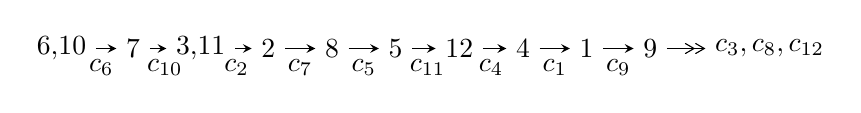
\begin{tikzpicture}[x=23pt, y=7pt]
	% node
	\node (A0) at (-1/8, 0) {6,10};
	\node (A1) at (1, 0) {7};
	\node (A2) at (33/16, 0) {3,11};
	\node (A3) at (25/8, 0) {2};
	\node (A4) at (33/8, 0) {8};
	\node (A5) at (41/8, 0) {5};
	\node (A6) at (49/8, 0) {12};
	\node (A7) at (57/8, 0) {4};
	\node (A8) at (65/8, 0) {1};
	\node (A9) at (73/8, 0) {9};
	\node (C1) at (1/2, -1) {$c_{6}$};
	\node (C2) at (3/2, -1) {$c_{10}$};
	\node (C3) at (21/8, -1) {$c_{2}$};
	\node (C4) at (29/8, -1) {$c_{7}$};
	\node (C5) at (37/8, -1) {$c_{5}$};
	\node (C6) at (45/8, -1) {$c_{11}$};
	\node (C7) at (53/8, -1) {$c_{4}$};
	\node (C8) at (61/8, -1) {$c_{1}$};
	\node (C9) at (69/8, -1) {$c_{9}$};
	\node (A10) at (11, 0) {$c_{3},c_{8},c_{12}$};

	% edge
	\draw[->,>=stealth]	
	(A0) edge (A1) (A1) edge (A2) (A2) edge (A3) (A3) edge (A4) (A4) edge (A5) (A5) edge (A6) (A6) edge (A7) (A7) edge (A8) (A8) edge (A9) ;
	\draw[->>,>={angle 60}]	
	(A9) edge (A10);
\end{tikzpicture} \\ 

\end{tabular} \\

\footnotetext{
The image of knot diagram is generated by the software ``\textbf{Draw programme}" developed by Andrew Bartholomew(\url{http://www.layer8.co.uk/maths/draw/index.htm\#Running-draw}), where we modified some parts for our purpose(\url{https://github.com/CATsTAILs/LinksPainter}).
}\phantom \\ \newline 
\centering \textbf{Ideals for irreducible components\footnotemark of $X_{\text{par}}$} 
 
\begin{align*}
I^u_{1}&=\langle 
2.68814\times10^{39} u^{31}+4.43259\times10^{39} u^{30}+\cdots+1.03715\times10^{39} b+8.81961\times10^{39},\\
\phantom{I^u_{1}}&\phantom{= \langle  }-2.68814\times10^{39} u^{31}-4.43259\times10^{39} u^{30}+\cdots+1.03715\times10^{39} a-9.85676\times10^{39},\;u^{32}+2 u^{31}+\cdots+3 u+1\rangle \\
I^u_{2}&=\langle 
-9.65086\times10^{81} u^{35}-1.35252\times10^{82} u^{34}+\cdots+5.32581\times10^{85} b+4.57159\times10^{85},\\
\phantom{I^u_{2}}&\phantom{= \langle  }-7.17774\times10^{84} u^{35}-2.27336\times10^{85} u^{34}+\cdots+7.05055\times10^{87} a+1.28066\times10^{88},\\
\phantom{I^u_{2}}&\phantom{= \langle  }u^{36}+2 u^{35}+\cdots-345 u+1721\rangle \\
I^u_{3}&=\langle 
-588 u^{14}-1117 u^{13}+\cdots+1513 b+3572,\;588 u^{14}+1117 u^{13}+\cdots+1513 a-2059,\\
\phantom{I^u_{3}}&\phantom{= \langle  }u^{15}+3 u^{14}+3 u^{13}-7 u^{11}-16 u^{10}-14 u^9+2 u^8+26 u^7+50 u^6+59 u^5+48 u^4+30 u^3+13 u^2+4 u+1\rangle \\
I^u_{4}&=\langle 
b,\;a-1,\;u-1\rangle \\
I^u_{5}&=\langle 
b,\;a- u-2,\;u^2+u-1\rangle \\
\\
\end{align*}
\raggedright * 5 irreducible components of $\dim_{\mathbb{C}}=0$, with total 86 representations.\\
\footnotetext{All coefficients of polynomials are rational numbers. But the coefficients are sometimes approximated in decimal forms when there is not enough margin.}
\newpage
\renewcommand{\arraystretch}{1}
\centering \section*{I. $I^u_{1}= \langle 2.69\times10^{39} u^{31}+4.43\times10^{39} u^{30}+\cdots+1.04\times10^{39} b+8.82\times10^{39},\;-2.69\times10^{39} u^{31}-4.43\times10^{39} u^{30}+\cdots+1.04\times10^{39} a-9.86\times10^{39},\;u^{32}+2 u^{31}+\cdots+3 u+1 \rangle$}
\flushleft \textbf{(i) Arc colorings}\\
\begin{tabular}{m{7pt} m{180pt} m{7pt} m{180pt} }
\flushright $a_{6}=$&$\begin{pmatrix}1\\0\end{pmatrix}$ \\
\flushright $a_{10}=$&$\begin{pmatrix}0\\u\end{pmatrix}$ \\
\flushright $a_{7}=$&$\begin{pmatrix}1\\u^2\end{pmatrix}$ \\
\flushright $a_{3}=$&$\begin{pmatrix}2.59186 u^{31}+4.27384 u^{30}+\cdots+0.0225842 u+9.50373\\-2.59186 u^{31}-4.27384 u^{30}+\cdots-0.0225842 u-8.50373\end{pmatrix}$ \\
\flushright $a_{11}=$&$\begin{pmatrix}- u\\u\end{pmatrix}$ \\
\flushright $a_{2}=$&$\begin{pmatrix}1\\-2.59186 u^{31}-4.27384 u^{30}+\cdots-0.0225842 u-8.50373\end{pmatrix}$ \\
\flushright $a_{8}=$&$\begin{pmatrix}-2.59186 u^{31}-4.27384 u^{30}+\cdots-0.0225842 u-7.50373\\0.934704 u^{31}+1.45438 u^{30}+\cdots+1.23689 u+2.26933\end{pmatrix}$ \\
\flushright $a_{5}=$&$\begin{pmatrix}3.21748 u^{31}+5.20620 u^{30}+\cdots+1.12168 u+10.8632\\-0.625617 u^{31}-0.932359 u^{30}+\cdots-1.09909 u-1.35945\end{pmatrix}$ \\
\flushright $a_{12}=$&$\begin{pmatrix}-0.835399 u^{31}-1.31731 u^{30}+\cdots-0.385321 u-1.44477\\-1.30325 u^{31}-2.20760 u^{30}+\cdots+2.32421 u-4.36458\end{pmatrix}$ \\
\flushright $a_{4}=$&$\begin{pmatrix}3.21748 u^{31}+5.20620 u^{30}+\cdots+1.12168 u+10.8632\\-0.182315 u^{31}-0.176177 u^{30}+\cdots-0.630287 u-0.130685\end{pmatrix}$ \\
\flushright $a_{1}=$&$\begin{pmatrix}1.47940 u^{31}+2.41530 u^{30}+\cdots-0.101041 u+4.07523\\0.504058 u^{31}+0.994655 u^{30}+\cdots-0.583979 u+1.83194\end{pmatrix}$ \\
\flushright $a_{9}=$&$\begin{pmatrix}-1.16297 u^{31}-1.83866 u^{30}+\cdots-0.347165 u-4.48853\\0.540348 u^{31}+0.679881 u^{30}+\cdots+0.438800 u+2.01562\end{pmatrix}$\\&\end{tabular}
\flushleft \textbf{(ii) Obstruction class $= -1$}\\~\\
\flushleft \textbf{(iii) Cusp Shapes $= 8.53130 u^{31}+14.3893 u^{30}+\cdots+9.88172 u+20.4373$}\\~\\
\newpage\renewcommand{\arraystretch}{1}
\flushleft \textbf{(iv) u-Polynomials at the component}\newline \\
\begin{tabular}{m{50pt}|m{274pt}}
Crossings & \hspace{64pt}u-Polynomials at each crossing \\
\hline $$\begin{aligned}c_{1},c_{3}\end{aligned}$$&$\begin{aligned}
&u^{32}-2 u^{30}+\cdots+6 u^2+1
\end{aligned}$\\
\hline $$\begin{aligned}c_{2},c_{5}\end{aligned}$$&$\begin{aligned}
&u^{32}-9 u^{31}+\cdots-12 u+9
\end{aligned}$\\
\hline $$\begin{aligned}c_{4}\end{aligned}$$&$\begin{aligned}
&u^{32}-2 u^{31}+\cdots+22 u+4
\end{aligned}$\\
\hline $$\begin{aligned}c_{6},c_{10}\end{aligned}$$&$\begin{aligned}
&u^{32}-2 u^{31}+\cdots-3 u+1
\end{aligned}$\\
\hline $$\begin{aligned}c_{7}\end{aligned}$$&$\begin{aligned}
&u^{32}+31 u^{31}+\cdots+1966080 u+131072
\end{aligned}$\\
\hline $$\begin{aligned}c_{8},c_{9},c_{12}\end{aligned}$$&$\begin{aligned}
&u^{32}-10 u^{31}+\cdots+24 u+9
\end{aligned}$\\
\hline $$\begin{aligned}c_{11}\end{aligned}$$&$\begin{aligned}
&u^{32}-2 u^{31}+\cdots-926 u+233
\end{aligned}$\\
\hline
\end{tabular}\\~\\
\newpage\renewcommand{\arraystretch}{1}
\flushleft \textbf{(v) Riley Polynomials at the component}\newline \\
\begin{tabular}{m{50pt}|m{274pt}}
Crossings & \hspace{64pt}Riley Polynomials at each crossing \\
\hline $$\begin{aligned}c_{1},c_{3}\end{aligned}$$&$\begin{aligned}
&y^{32}-4 y^{31}+\cdots+12 y+1
\end{aligned}$\\
\hline $$\begin{aligned}c_{2},c_{5}\end{aligned}$$&$\begin{aligned}
&y^{32}+13 y^{31}+\cdots-630 y+81
\end{aligned}$\\
\hline $$\begin{aligned}c_{4}\end{aligned}$$&$\begin{aligned}
&y^{32}+2 y^{31}+\cdots-188 y+16
\end{aligned}$\\
\hline $$\begin{aligned}c_{6},c_{10}\end{aligned}$$&$\begin{aligned}
&y^{32}-40 y^{31}+\cdots-11 y+1
\end{aligned}$\\
\hline $$\begin{aligned}c_{7}\end{aligned}$$&$\begin{aligned}
&y^{32}+3 y^{31}+\cdots-51539607552 y+17179869184
\end{aligned}$\\
\hline $$\begin{aligned}c_{8},c_{9},c_{12}\end{aligned}$$&$\begin{aligned}
&y^{32}-34 y^{31}+\cdots+1260 y+81
\end{aligned}$\\
\hline $$\begin{aligned}c_{11}\end{aligned}$$&$\begin{aligned}
&y^{32}+30 y^{31}+\cdots+118794 y+54289
\end{aligned}$\\
\hline
\end{tabular}\\~\\
\newpage\flushleft \textbf{(vi) Complex Volumes and Cusp Shapes}
$$\begin{array}{c|c|c}  
\text{Solutions to }I^u_{1}& \I (\text{vol} + \sqrt{-1}CS) & \text{Cusp shape}\\
 \hline 
\begin{aligned}
u &= -0.727787 + 0.359428 I \\
a &= \phantom{-}1.50645 + 0.30685 I \\
b &= -0.506447 - 0.306846 I\end{aligned}
 & \phantom{-}3.01151 - 0.12453 I & \phantom{-}2.01930 - 0.65952 I \\ \hline\begin{aligned}
u &= -0.727787 - 0.359428 I \\
a &= \phantom{-}1.50645 - 0.30685 I \\
b &= -0.506447 + 0.306846 I\end{aligned}
 & \phantom{-}3.01151 + 0.12453 I & \phantom{-}2.01930 + 0.65952 I \\ \hline\begin{aligned}
u &= -1.088820 + 0.491186 I \\
a &= \phantom{-}0.429547 + 0.223085 I \\
b &= \phantom{-}0.570453 - 0.223085 I\end{aligned}
 & \phantom{-}2.15764 - 0.43132 I & \phantom{-}3.87708 + 2.50521 I \\ \hline\begin{aligned}
u &= -1.088820 - 0.491186 I \\
a &= \phantom{-}0.429547 - 0.223085 I \\
b &= \phantom{-}0.570453 + 0.223085 I\end{aligned}
 & \phantom{-}2.15764 + 0.43132 I & \phantom{-}3.87708 - 2.50521 I \\ \hline\begin{aligned}
u &= \phantom{-}0.123243 + 0.684919 I \\
a &= \phantom{-}1.074160 + 0.889657 I \\
b &= -0.074156 - 0.889657 I\end{aligned}
 & \phantom{-}1.24572 - 1.59798 I & -0.69901 + 4.34280 I \\ \hline\begin{aligned}
u &= \phantom{-}0.123243 - 0.684919 I \\
a &= \phantom{-}1.074160 - 0.889657 I \\
b &= -0.074156 + 0.889657 I\end{aligned}
 & \phantom{-}1.24572 + 1.59798 I & -0.69901 - 4.34280 I \\ \hline\begin{aligned}
u &= -0.181903 + 0.562687 I \\
a &= \phantom{-}1.76402 - 0.20287 I \\
b &= -0.764020 + 0.202871 I\end{aligned}
 & \phantom{-}3.20927 + 1.51045 I & \phantom{-}1.61636 - 4.36798 I \\ \hline\begin{aligned}
u &= -0.181903 - 0.562687 I \\
a &= \phantom{-}1.76402 + 0.20287 I \\
b &= -0.764020 - 0.202871 I\end{aligned}
 & \phantom{-}3.20927 - 1.51045 I & \phantom{-}1.61636 + 4.36798 I \\ \hline\begin{aligned}
u &= \phantom{-}0.570063 + 0.113911 I \\
a &= \phantom{-}1.10156 - 1.54628 I \\
b &= -0.10156 + 1.54628 I\end{aligned}
 & \phantom{-}9.84884 + 5.18562 I & \phantom{-}1.41138 - 2.71485 I \\ \hline\begin{aligned}
u &= \phantom{-}0.570063 - 0.113911 I \\
a &= \phantom{-}1.10156 + 1.54628 I \\
b &= -0.10156 - 1.54628 I\end{aligned}
 & \phantom{-}9.84884 - 5.18562 I & \phantom{-}1.41138 + 2.71485 I\\
 \hline 
 \end{array}$$\newpage$$\begin{array}{c|c|c}  
\text{Solutions to }I^u_{1}& \I (\text{vol} + \sqrt{-1}CS) & \text{Cusp shape}\\
 \hline 
\begin{aligned}
u &= \phantom{-}0.097390 + 0.483297 I \\
a &= \phantom{-}1.44762 - 1.17049 I \\
b &= -0.447624 + 1.170490 I\end{aligned}
 & \phantom{-}5.83833 + 4.06602 I & \phantom{-}6.43607 - 3.22823 I \\ \hline\begin{aligned}
u &= \phantom{-}0.097390 - 0.483297 I \\
a &= \phantom{-}1.44762 + 1.17049 I \\
b &= -0.447624 - 1.170490 I\end{aligned}
 & \phantom{-}5.83833 - 4.06602 I & \phantom{-}6.43607 + 3.22823 I \\ \hline\begin{aligned}
u &= -1.30092 + 0.76651 I \\
a &= \phantom{-}0.565351 - 1.100220 I \\
b &= \phantom{-}0.434649 + 1.100220 I\end{aligned}
 & \phantom{-}4.66242 - 4.30535 I & \phantom{-0.000000 } 0 \\ \hline\begin{aligned}
u &= -1.30092 - 0.76651 I \\
a &= \phantom{-}0.565351 + 1.100220 I \\
b &= \phantom{-}0.434649 - 1.100220 I\end{aligned}
 & \phantom{-}4.66242 + 4.30535 I & \phantom{-0.000000 } 0 \\ \hline\begin{aligned}
u &= -1.58301 + 0.10612 I \\
a &= -0.040653 - 0.769050 I \\
b &= \phantom{-}1.040650 + 0.769050 I\end{aligned}
 & -5.78170 + 5.02185 I & \phantom{-0.000000 } 0 \\ \hline\begin{aligned}
u &= -1.58301 - 0.10612 I \\
a &= -0.040653 + 0.769050 I \\
b &= \phantom{-}1.040650 - 0.769050 I\end{aligned}
 & -5.78170 - 5.02185 I & \phantom{-0.000000 } 0 \\ \hline\begin{aligned}
u &= \phantom{-}1.59789 + 0.07572 I \\
a &= \phantom{-}0.152087 + 0.822987 I \\
b &= \phantom{-}0.847913 - 0.822987 I\end{aligned}
 & -4.90783 - 0.17419 I & \phantom{-0.000000 } 0 \\ \hline\begin{aligned}
u &= \phantom{-}1.59789 - 0.07572 I \\
a &= \phantom{-}0.152087 - 0.822987 I \\
b &= \phantom{-}0.847913 + 0.822987 I\end{aligned}
 & -4.90783 + 0.17419 I & \phantom{-0.000000 } 0 \\ \hline\begin{aligned}
u &= \phantom{-}1.59468 + 0.12683 I \\
a &= -0.176743 + 0.703049 I \\
b &= \phantom{-}1.176740 - 0.703049 I\end{aligned}
 & \phantom{-}0.33699 - 8.78781 I & \phantom{-0.000000 } 0 \\ \hline\begin{aligned}
u &= \phantom{-}1.59468 - 0.12683 I \\
a &= -0.176743 - 0.703049 I \\
b &= \phantom{-}1.176740 + 0.703049 I\end{aligned}
 & \phantom{-}0.33699 + 8.78781 I & \phantom{-0.000000 } 0\\
 \hline 
 \end{array}$$\newpage$$\begin{array}{c|c|c}  
\text{Solutions to }I^u_{1}& \I (\text{vol} + \sqrt{-1}CS) & \text{Cusp shape}\\
 \hline 
\begin{aligned}
u &= \phantom{-}0.224964 + 0.303301 I \\
a &= \phantom{-}1.60702 + 0.01432 I \\
b &= -0.607019 - 0.014324 I\end{aligned}
 & -1.277390 - 0.391091 I & -8.45483 + 1.44760 I \\ \hline\begin{aligned}
u &= \phantom{-}0.224964 - 0.303301 I \\
a &= \phantom{-}1.60702 - 0.01432 I \\
b &= -0.607019 + 0.014324 I\end{aligned}
 & -1.277390 + 0.391091 I & -8.45483 - 1.44760 I \\ \hline\begin{aligned}
u &= -0.329013 + 0.018023 I \\
a &= \phantom{-}1.16462 + 1.38080 I \\
b &= -0.164619 - 1.380800 I\end{aligned}
 & \phantom{-}3.64918 - 3.45629 I & -10.02596 + 4.62950 I \\ \hline\begin{aligned}
u &= -0.329013 - 0.018023 I \\
a &= \phantom{-}1.16462 - 1.38080 I \\
b &= -0.164619 + 1.380800 I\end{aligned}
 & \phantom{-}3.64918 + 3.45629 I & -10.02596 - 4.62950 I \\ \hline\begin{aligned}
u &= -1.74543 + 0.37989 I \\
a &= \phantom{-}0.439100 + 0.949102 I \\
b &= \phantom{-}0.560900 - 0.949102 I\end{aligned}
 & \phantom{-}4.10800 + 2.16881 I & \phantom{-0.000000 } 0 \\ \hline\begin{aligned}
u &= -1.74543 - 0.37989 I \\
a &= \phantom{-}0.439100 - 0.949102 I \\
b &= \phantom{-}0.560900 + 0.949102 I\end{aligned}
 & \phantom{-}4.10800 - 2.16881 I & \phantom{-0.000000 } 0 \\ \hline\begin{aligned}
u &= \phantom{-}1.71462 + 0.67318 I \\
a &= \phantom{-}0.120504 - 1.186710 I \\
b &= \phantom{-}0.87950 + 1.18671 I\end{aligned}
 & \phantom{-}1.9107 - 16.1447 I & \phantom{-0.000000 } 0 \\ \hline\begin{aligned}
u &= \phantom{-}1.71462 - 0.67318 I \\
a &= \phantom{-}0.120504 + 1.186710 I \\
b &= \phantom{-}0.87950 - 1.18671 I\end{aligned}
 & \phantom{-}1.9107 + 16.1447 I & \phantom{-0.000000 } 0 \\ \hline\begin{aligned}
u &= -1.72533 + 0.66821 I \\
a &= \phantom{-}0.136057 + 1.096830 I \\
b &= \phantom{-}0.863943 - 1.096830 I\end{aligned}
 & -4.72526 + 11.94950 I & \phantom{-0.000000 } 0 \\ \hline\begin{aligned}
u &= -1.72533 - 0.66821 I \\
a &= \phantom{-}0.136057 - 1.096830 I \\
b &= \phantom{-}0.863943 + 1.096830 I\end{aligned}
 & -4.72526 - 11.94950 I & \phantom{-0.000000 } 0\\
 \hline 
 \end{array}$$\newpage$$\begin{array}{c|c|c}  
\text{Solutions to }I^u_{1}& \I (\text{vol} + \sqrt{-1}CS) & \text{Cusp shape}\\
 \hline 
\begin{aligned}
u &= \phantom{-}1.75936 + 0.67100 I \\
a &= \phantom{-}0.209299 - 0.991283 I \\
b &= \phantom{-}0.790701 + 0.991283 I\end{aligned}
 & -4.36968 - 6.32073 I & \phantom{-0.000000 } 0 \\ \hline\begin{aligned}
u &= \phantom{-}1.75936 - 0.67100 I \\
a &= \phantom{-}0.209299 + 0.991283 I \\
b &= \phantom{-}0.790701 - 0.991283 I\end{aligned}
 & -4.36968 + 6.32073 I & \phantom{-0.000000 } 0\\
 \hline 
 \end{array}$$\newpage\newpage\renewcommand{\arraystretch}{1}
\centering \section*{II. $I^u_{2}= \langle -9.65\times10^{81} u^{35}-1.35\times10^{82} u^{34}+\cdots+5.33\times10^{85} b+4.57\times10^{85},\;-7.18\times10^{84} u^{35}-2.27\times10^{85} u^{34}+\cdots+7.05\times10^{87} a+1.28\times10^{88},\;u^{36}+2 u^{35}+\cdots-345 u+1721 \rangle$}
\flushleft \textbf{(i) Arc colorings}\\
\begin{tabular}{m{7pt} m{180pt} m{7pt} m{180pt} }
\flushright $a_{6}=$&$\begin{pmatrix}1\\0\end{pmatrix}$ \\
\flushright $a_{10}=$&$\begin{pmatrix}0\\u\end{pmatrix}$ \\
\flushright $a_{7}=$&$\begin{pmatrix}1\\u^2\end{pmatrix}$ \\
\flushright $a_{3}=$&$\begin{pmatrix}0.00101804 u^{35}+0.00322437 u^{34}+\cdots-3.03218 u-1.81639\\0.000181209 u^{35}+0.000253957 u^{34}+\cdots-1.69137 u-0.858384\end{pmatrix}$ \\
\flushright $a_{11}=$&$\begin{pmatrix}- u\\u\end{pmatrix}$ \\
\flushright $a_{2}=$&$\begin{pmatrix}0.00119925 u^{35}+0.00347833 u^{34}+\cdots-4.72355 u-2.67478\\0.000181209 u^{35}+0.000253957 u^{34}+\cdots-1.69137 u-0.858384\end{pmatrix}$ \\
\flushright $a_{8}=$&$\begin{pmatrix}0.00119925 u^{35}+0.00347833 u^{34}+\cdots-4.72355 u-1.67478\\0.000181209 u^{35}+0.000253957 u^{34}+\cdots-1.69137 u-0.858384\end{pmatrix}$ \\
\flushright $a_{5}=$&$\begin{pmatrix}0.00122718 u^{35}+0.00328059 u^{34}+\cdots-1.81467 u+0.516616\\-0.000330064 u^{35}-0.00139754 u^{34}+\cdots+0.178060 u+0.705552\end{pmatrix}$ \\
\flushright $a_{12}=$&$\begin{pmatrix}0.000158903 u^{35}+0.00143193 u^{34}+\cdots-0.847012 u-2.41702\\0.00166960 u^{35}+0.00517909 u^{34}+\cdots-0.901484 u-2.62550\end{pmatrix}$ \\
\flushright $a_{4}=$&$\begin{pmatrix}0.00122718 u^{35}+0.00328059 u^{34}+\cdots-1.81467 u+0.516616\\0.000525501 u^{35}+0.00101205 u^{34}+\cdots-1.64888 u-0.716369\end{pmatrix}$ \\
\flushright $a_{1}=$&$\begin{pmatrix}0.000933234 u^{35}+0.00308935 u^{34}+\cdots+1.23389 u-4.21048\\0.00191049 u^{35}+0.00584877 u^{34}+\cdots-0.657755 u-3.18542\end{pmatrix}$ \\
\flushright $a_{9}=$&$\begin{pmatrix}0.000694411 u^{35}+0.00104134 u^{34}+\cdots-2.62227 u+2.26900\\-0.000527487 u^{35}-0.00143426 u^{34}+\cdots+0.446693 u+1.57292\end{pmatrix}$\\&\end{tabular}
\flushleft \textbf{(ii) Obstruction class $= -1$}\\~\\
\flushleft \textbf{(iii) Cusp Shapes $= 0.00480094 u^{35}+0.0143993 u^{34}+\cdots-10.3752 u-14.3937$}\\~\\
\newpage\renewcommand{\arraystretch}{1}
\flushleft \textbf{(iv) u-Polynomials at the component}\newline \\
\begin{tabular}{m{50pt}|m{274pt}}
Crossings & \hspace{64pt}u-Polynomials at each crossing \\
\hline $$\begin{aligned}c_{1},c_{3}\end{aligned}$$&$\begin{aligned}
&u^{36}-3 u^{35}+\cdots-26 u+1
\end{aligned}$\\
\hline $$\begin{aligned}c_{2},c_{5}\end{aligned}$$&$\begin{aligned}
&(u^{18}+7 u^{17}+\cdots+3 u+2)^{2}
\end{aligned}$\\
\hline $$\begin{aligned}c_{4}\end{aligned}$$&$\begin{aligned}
&u^{36}+4 u^{34}+\cdots-81 u+7
\end{aligned}$\\
\hline $$\begin{aligned}c_{6},c_{10}\end{aligned}$$&$\begin{aligned}
&u^{36}-2 u^{35}+\cdots+345 u+1721
\end{aligned}$\\
\hline $$\begin{aligned}c_{7}\end{aligned}$$&$\begin{aligned}
&(u-1)^{36}
\end{aligned}$\\
\hline $$\begin{aligned}c_{8},c_{9},c_{12}\end{aligned}$$&$\begin{aligned}
&(u^{18}+2 u^{17}+\cdots+2 u+1)^{2}
\end{aligned}$\\
\hline $$\begin{aligned}c_{11}\end{aligned}$$&$\begin{aligned}
&u^{36}-2 u^{35}+\cdots-107951 u+18799
\end{aligned}$\\
\hline
\end{tabular}\\~\\
\newpage\renewcommand{\arraystretch}{1}
\flushleft \textbf{(v) Riley Polynomials at the component}\newline \\
\begin{tabular}{m{50pt}|m{274pt}}
Crossings & \hspace{64pt}Riley Polynomials at each crossing \\
\hline $$\begin{aligned}c_{1},c_{3}\end{aligned}$$&$\begin{aligned}
&y^{36}+13 y^{35}+\cdots-238 y+1
\end{aligned}$\\
\hline $$\begin{aligned}c_{2},c_{5}\end{aligned}$$&$\begin{aligned}
&(y^{18}+3 y^{17}+\cdots+27 y+4)^{2}
\end{aligned}$\\
\hline $$\begin{aligned}c_{4}\end{aligned}$$&$\begin{aligned}
&y^{36}+8 y^{35}+\cdots+24785 y+49
\end{aligned}$\\
\hline $$\begin{aligned}c_{6},c_{10}\end{aligned}$$&$\begin{aligned}
&y^{36}-24 y^{35}+\cdots-23369735 y+2961841
\end{aligned}$\\
\hline $$\begin{aligned}c_{7}\end{aligned}$$&$\begin{aligned}
&(y-1)^{36}
\end{aligned}$\\
\hline $$\begin{aligned}c_{8},c_{9},c_{12}\end{aligned}$$&$\begin{aligned}
&(y^{18}-18 y^{17}+\cdots+6 y+1)^{2}
\end{aligned}$\\
\hline $$\begin{aligned}c_{11}\end{aligned}$$&$\begin{aligned}
&y^{36}+20 y^{35}+\cdots+3655697641 y+353402401
\end{aligned}$\\
\hline
\end{tabular}\\~\\
\newpage\flushleft \textbf{(vi) Complex Volumes and Cusp Shapes}
$$\begin{array}{c|c|c}  
\text{Solutions to }I^u_{2}& \I (\text{vol} + \sqrt{-1}CS) & \text{Cusp shape}\\
 \hline 
\begin{aligned}
u &= \phantom{-}0.951328 + 0.265633 I \\
a &= -1.00770 + 1.00856 I \\
b &= -0.799005 - 0.432049 I\end{aligned}
 & -0.749045 - 0.267600 I & -5.91340 + 2.02101 I \\ \hline\begin{aligned}
u &= \phantom{-}0.951328 - 0.265633 I \\
a &= -1.00770 - 1.00856 I \\
b &= -0.799005 + 0.432049 I\end{aligned}
 & -0.749045 + 0.267600 I & -5.91340 - 2.02101 I \\ \hline\begin{aligned}
u &= -0.648013 + 0.675517 I \\
a &= \phantom{-}0.627478 - 0.216336 I \\
b &= \phantom{-}0.186015 - 0.679590 I\end{aligned}
 & \phantom{-}1.71945 - 1.37809 I & \phantom{-}3.91287 - 1.41254 I \\ \hline\begin{aligned}
u &= -0.648013 - 0.675517 I \\
a &= \phantom{-}0.627478 + 0.216336 I \\
b &= \phantom{-}0.186015 + 0.679590 I\end{aligned}
 & \phantom{-}1.71945 + 1.37809 I & \phantom{-}3.91287 + 1.41254 I \\ \hline\begin{aligned}
u &= \phantom{-}0.823523 + 0.347145 I \\
a &= -0.079307 + 0.626674 I \\
b &= \phantom{-}0.172943 + 0.911158 I\end{aligned}
 & \phantom{-}8.82842 + 4.51784 I & \phantom{-}4.44915 - 1.04065 I \\ \hline\begin{aligned}
u &= \phantom{-}0.823523 - 0.347145 I \\
a &= -0.079307 - 0.626674 I \\
b &= \phantom{-}0.172943 - 0.911158 I\end{aligned}
 & \phantom{-}8.82842 - 4.51784 I & \phantom{-}4.44915 + 1.04065 I \\ \hline\begin{aligned}
u &= \phantom{-}0.078059 + 1.130100 I \\
a &= \phantom{-}0.369477 + 1.291370 I \\
b &= \phantom{-}0.186015 - 0.679590 I\end{aligned}
 & \phantom{-}1.71945 - 1.37809 I & \phantom{-}3.91287 - 1.41254 I \\ \hline\begin{aligned}
u &= \phantom{-}0.078059 - 1.130100 I \\
a &= \phantom{-}0.369477 - 1.291370 I \\
b &= \phantom{-}0.186015 + 0.679590 I\end{aligned}
 & \phantom{-}1.71945 + 1.37809 I & \phantom{-}3.91287 + 1.41254 I \\ \hline\begin{aligned}
u &= -1.207030 + 0.342060 I \\
a &= -0.344195 - 1.035250 I \\
b &= -1.007410 + 0.797418 I\end{aligned}
 & -4.69253 + 2.67585 I & -11.48246 + 0.04874 I \\ \hline\begin{aligned}
u &= -1.207030 - 0.342060 I \\
a &= -0.344195 + 1.035250 I \\
b &= -1.007410 - 0.797418 I\end{aligned}
 & -4.69253 - 2.67585 I & -11.48246 - 0.04874 I\\
 \hline 
 \end{array}$$\newpage$$\begin{array}{c|c|c}  
\text{Solutions to }I^u_{2}& \I (\text{vol} + \sqrt{-1}CS) & \text{Cusp shape}\\
 \hline 
\begin{aligned}
u &= \phantom{-}1.304090 + 0.242334 I \\
a &= -0.172903 + 0.923671 I \\
b &= -1.20068 - 1.01012 I\end{aligned}
 & -1.01052 - 4.22577 I & -7.20649 + 4.92260 I \\ \hline\begin{aligned}
u &= \phantom{-}1.304090 - 0.242334 I \\
a &= -0.172903 - 0.923671 I \\
b &= -1.20068 + 1.01012 I\end{aligned}
 & -1.01052 + 4.22577 I & -7.20649 - 4.92260 I \\ \hline\begin{aligned}
u &= \phantom{-}1.339670 + 0.120163 I \\
a &= -0.297280 + 0.744568 I \\
b &= -0.80875 - 1.24243 I\end{aligned}
 & \phantom{-}1.72404 - 6.10285 I & -0.03303 + 7.78532 I \\ \hline\begin{aligned}
u &= \phantom{-}1.339670 - 0.120163 I \\
a &= -0.297280 - 0.744568 I \\
b &= -0.80875 + 1.24243 I\end{aligned}
 & \phantom{-}1.72404 + 6.10285 I & -0.03303 - 7.78532 I \\ \hline\begin{aligned}
u &= -0.456738 + 1.298950 I \\
a &= -0.13350 - 1.55902 I \\
b &= \phantom{-}0.172943 + 0.911158 I\end{aligned}
 & \phantom{-}8.82842 + 4.51784 I & \phantom{-}4.44915 - 1.04065 I \\ \hline\begin{aligned}
u &= -0.456738 - 1.298950 I \\
a &= -0.13350 + 1.55902 I \\
b &= \phantom{-}0.172943 - 0.911158 I\end{aligned}
 & \phantom{-}8.82842 - 4.51784 I & \phantom{-}4.44915 + 1.04065 I \\ \hline\begin{aligned}
u &= -1.41435 + 0.18193 I \\
a &= -0.123524 - 0.807920 I \\
b &= -0.92905 + 1.08318 I\end{aligned}
 & -3.82636 + 4.39821 I & -4.26128 - 12.11852 I \\ \hline\begin{aligned}
u &= -1.41435 - 0.18193 I \\
a &= -0.123524 + 0.807920 I \\
b &= -0.92905 - 1.08318 I\end{aligned}
 & -3.82636 - 4.39821 I & -4.26128 + 12.11852 I \\ \hline\begin{aligned}
u &= \phantom{-}0.329048 + 0.415115 I \\
a &= \phantom{-}2.16953 + 1.12232 I \\
b &= \phantom{-}0.370956 + 0.584694 I\end{aligned}
 & \phantom{-}1.15682 - 3.56504 I & -0.39209 + 9.87971 I \\ \hline\begin{aligned}
u &= \phantom{-}0.329048 - 0.415115 I \\
a &= \phantom{-}2.16953 - 1.12232 I \\
b &= \phantom{-}0.370956 - 0.584694 I\end{aligned}
 & \phantom{-}1.15682 + 3.56504 I & -0.39209 - 9.87971 I\\
 \hline 
 \end{array}$$\newpage$$\begin{array}{c|c|c}  
\text{Solutions to }I^u_{2}& \I (\text{vol} + \sqrt{-1}CS) & \text{Cusp shape}\\
 \hline 
\begin{aligned}
u &= \phantom{-}1.43862 + 0.58080 I \\
a &= \phantom{-}0.039810 + 1.315730 I \\
b &= -0.92905 - 1.08318 I\end{aligned}
 & -3.82636 - 4.39821 I & -4.26128 + 12.11852 I \\ \hline\begin{aligned}
u &= \phantom{-}1.43862 - 0.58080 I \\
a &= \phantom{-}0.039810 - 1.315730 I \\
b &= -0.92905 + 1.08318 I\end{aligned}
 & -3.82636 + 4.39821 I & -4.26128 - 12.11852 I \\ \hline\begin{aligned}
u &= -0.353911 + 0.263917 I \\
a &= \phantom{-}1.82923 - 2.67302 I \\
b &= \phantom{-}0.514983 - 0.621068 I\end{aligned}
 & \phantom{-}7.54180 + 7.47357 I & \phantom{-}0.42672 - 8.56588 I \\ \hline\begin{aligned}
u &= -0.353911 - 0.263917 I \\
a &= \phantom{-}1.82923 + 2.67302 I \\
b &= \phantom{-}0.514983 + 0.621068 I\end{aligned}
 & \phantom{-}7.54180 - 7.47357 I & \phantom{-}0.42672 + 8.56588 I \\ \hline\begin{aligned}
u &= \phantom{-}0.12734 + 1.61628 I \\
a &= -0.099767 - 0.766912 I \\
b &= \phantom{-}0.370956 + 0.584694 I\end{aligned}
 & \phantom{-}1.15682 - 3.56504 I & -0.39209 + 9.87971 I \\ \hline\begin{aligned}
u &= \phantom{-}0.12734 - 1.61628 I \\
a &= -0.099767 + 0.766912 I \\
b &= \phantom{-}0.370956 - 0.584694 I\end{aligned}
 & \phantom{-}1.15682 + 3.56504 I & -0.39209 - 9.87971 I \\ \hline\begin{aligned}
u &= -1.42189 + 0.79988 I \\
a &= \phantom{-}0.05695 - 1.58085 I \\
b &= -0.80875 + 1.24243 I\end{aligned}
 & \phantom{-}1.72404 + 6.10285 I & \phantom{-0.000000 } 0. - 7.78532 I \\ \hline\begin{aligned}
u &= -1.42189 - 0.79988 I \\
a &= \phantom{-}0.05695 + 1.58085 I \\
b &= -0.80875 - 1.24243 I\end{aligned}
 & \phantom{-}1.72404 - 6.10285 I & \phantom{-0.000000 -}0. + 7.78532 I \\ \hline\begin{aligned}
u &= \phantom{-}1.71277 + 0.17526 I \\
a &= \phantom{-}0.289764 + 0.671140 I \\
b &= -1.007410 - 0.797418 I\end{aligned}
 & -4.69253 - 2.67585 I & -11.48246 + 0. I\phantom{ +0.000000I} \\ \hline\begin{aligned}
u &= \phantom{-}1.71277 - 0.17526 I \\
a &= \phantom{-}0.289764 - 0.671140 I \\
b &= -1.007410 + 0.797418 I\end{aligned}
 & -4.69253 + 2.67585 I & -11.48246 + 0. I\phantom{ +0.000000I}\\
 \hline 
 \end{array}$$\newpage$$\begin{array}{c|c|c}  
\text{Solutions to }I^u_{2}& \I (\text{vol} + \sqrt{-1}CS) & \text{Cusp shape}\\
 \hline 
\begin{aligned}
u &= \phantom{-}0.03972 + 1.78449 I \\
a &= -0.371574 + 0.822587 I \\
b &= \phantom{-}0.514983 - 0.621068 I\end{aligned}
 & \phantom{-}7.54180 + 7.47357 I & \phantom{-0.000000 } 0. - 8.56588 I \\ \hline\begin{aligned}
u &= \phantom{-}0.03972 - 1.78449 I \\
a &= -0.371574 - 0.822587 I \\
b &= \phantom{-}0.514983 + 0.621068 I\end{aligned}
 & \phantom{-}7.54180 - 7.47357 I & \phantom{-0.000000 -}0. + 8.56588 I \\ \hline\begin{aligned}
u &= -1.77033 + 0.44561 I \\
a &= \phantom{-}0.475535 - 1.055760 I \\
b &= -1.20068 + 1.01012 I\end{aligned}
 & -1.01052 + 4.22577 I & \phantom{-0.000000 } 0. - 4.92260 I \\ \hline\begin{aligned}
u &= -1.77033 - 0.44561 I \\
a &= \phantom{-}0.475535 + 1.055760 I \\
b &= -1.20068 - 1.01012 I\end{aligned}
 & -1.01052 - 4.22577 I & \phantom{-0.000000 -}0. + 4.92260 I \\ \hline\begin{aligned}
u &= -1.87191 + 0.06853 I \\
a &= \phantom{-}0.296661 + 0.271754 I \\
b &= -0.799005 - 0.432049 I\end{aligned}
 & -0.749045 - 0.267600 I & \phantom{-0.000000 } 0 \\ \hline\begin{aligned}
u &= -1.87191 - 0.06853 I \\
a &= \phantom{-}0.296661 - 0.271754 I \\
b &= -0.799005 + 0.432049 I\end{aligned}
 & -0.749045 + 0.267600 I & \phantom{-0.000000 } 0\\
 \hline 
 \end{array}$$\newpage\newpage\renewcommand{\arraystretch}{1}
\centering \section*{III. $I^u_{3}= \langle -588 u^{14}-1117 u^{13}+\cdots+1513 b+3572,\;588 u^{14}+1117 u^{13}+\cdots+1513 a-2059,\;u^{15}+3 u^{14}+\cdots+4 u+1 \rangle$}
\flushleft \textbf{(i) Arc colorings}\\
\begin{tabular}{m{7pt} m{180pt} m{7pt} m{180pt} }
\flushright $a_{6}=$&$\begin{pmatrix}1\\0\end{pmatrix}$ \\
\flushright $a_{10}=$&$\begin{pmatrix}0\\u\end{pmatrix}$ \\
\flushright $a_{7}=$&$\begin{pmatrix}1\\u^2\end{pmatrix}$ \\
\flushright $a_{3}=$&$\begin{pmatrix}-0.388632 u^{14}-0.738268 u^{13}+\cdots+5.77859 u+1.36087\\0.388632 u^{14}+0.738268 u^{13}+\cdots-5.77859 u-2.36087\end{pmatrix}$ \\
\flushright $a_{11}=$&$\begin{pmatrix}- u\\u\end{pmatrix}$ \\
\flushright $a_{2}=$&$\begin{pmatrix}-1\\0.388632 u^{14}+0.738268 u^{13}+\cdots-5.77859 u-2.36087\end{pmatrix}$ \\
\flushright $a_{8}=$&$\begin{pmatrix}-0.388632 u^{14}-0.738268 u^{13}+\cdots+5.77859 u+3.36087\\0.815598 u^{14}+1.94052 u^{13}+\cdots+7.27759 u+1.09980\end{pmatrix}$ \\
\flushright $a_{5}=$&$\begin{pmatrix}1.51091 u^{14}+3.39061 u^{13}+\cdots+0.177132 u-0.688698\\-1.12227 u^{14}-2.65235 u^{13}+\cdots-5.95572 u-0.672174\end{pmatrix}$ \\
\flushright $a_{12}=$&$\begin{pmatrix}-0.881031 u^{14}-2.28420 u^{13}+\cdots-5.34038 u-0.967614\\-0.688698 u^{14}-2.57700 u^{13}+\cdots-5.30734 u-0.931923\end{pmatrix}$ \\
\flushright $a_{4}=$&$\begin{pmatrix}1.51091 u^{14}+3.39061 u^{13}+\cdots+0.177132 u-0.688698\\-0.967614 u^{14}-2.02181 u^{13}+\cdots-2.89822 u+0.469927\end{pmatrix}$ \\
\flushright $a_{1}=$&$\begin{pmatrix}0.747521 u^{14}+2.04759 u^{13}+\cdots-3.22208 u-2.47984\\-1.99802 u^{14}-4.83807 u^{13}+\cdots-5.42234 u-0.216127\end{pmatrix}$ \\
\flushright $a_{9}=$&$\begin{pmatrix}1.55254 u^{14}+3.79114 u^{13}+\cdots+4.30800 u+1.77264\\-0.0647720 u^{14}+1.04362 u^{13}+\cdots+10.7964 u+3.06015\end{pmatrix}$\\&\end{tabular}
\flushleft \textbf{(ii) Obstruction class $= 1$}\\~\\
\flushleft \textbf{(iii) Cusp Shapes $= -\frac{11241}{1513} u^{14}-\frac{26858}{1513} u^{13}+\cdots-\frac{17389}{1513} u+\frac{5791}{1513}$}\\~\\
\newpage\renewcommand{\arraystretch}{1}
\flushleft \textbf{(iv) u-Polynomials at the component}\newline \\
\begin{tabular}{m{50pt}|m{274pt}}
Crossings & \hspace{64pt}u-Polynomials at each crossing \\
\hline $$\begin{aligned}c_{1},c_{3}\end{aligned}$$&$\begin{aligned}
&u^{15}+u^{14}+\cdots- u-1
\end{aligned}$\\
\hline $$\begin{aligned}c_{2}\end{aligned}$$&$\begin{aligned}
&u^{15}-6 u^{14}+\cdots+19 u-5
\end{aligned}$\\
\hline $$\begin{aligned}c_{4}\end{aligned}$$&$\begin{aligned}
&u^{15}- u^{14}+\cdots-2 u+1
\end{aligned}$\\
\hline $$\begin{aligned}c_{5}\end{aligned}$$&$\begin{aligned}
&u^{15}+6 u^{14}+\cdots+19 u+5
\end{aligned}$\\
\hline $$\begin{aligned}c_{6}\end{aligned}$$&$\begin{aligned}
&u^{15}+3 u^{14}+\cdots+4 u+1
\end{aligned}$\\
\hline $$\begin{aligned}c_{7}\end{aligned}$$&$\begin{aligned}
&u^{15}+3 u^{14}+\cdots+19 u+7
\end{aligned}$\\
\hline $$\begin{aligned}c_{8},c_{9}\end{aligned}$$&$\begin{aligned}
&u^{15}-3 u^{14}+\cdots-5 u+1
\end{aligned}$\\
\hline $$\begin{aligned}c_{10}\end{aligned}$$&$\begin{aligned}
&u^{15}-3 u^{14}+\cdots+4 u-1
\end{aligned}$\\
\hline $$\begin{aligned}c_{11}\end{aligned}$$&$\begin{aligned}
&u^{15}- u^{14}+\cdots+37 u-7
\end{aligned}$\\
\hline $$\begin{aligned}c_{12}\end{aligned}$$&$\begin{aligned}
&u^{15}+3 u^{14}+\cdots-5 u-1
\end{aligned}$\\
\hline
\end{tabular}\\~\\
\newpage\renewcommand{\arraystretch}{1}
\flushleft \textbf{(v) Riley Polynomials at the component}\newline \\
\begin{tabular}{m{50pt}|m{274pt}}
Crossings & \hspace{64pt}Riley Polynomials at each crossing \\
\hline $$\begin{aligned}c_{1},c_{3}\end{aligned}$$&$\begin{aligned}
&y^{15}+9 y^{14}+\cdots- y-1
\end{aligned}$\\
\hline $$\begin{aligned}c_{2},c_{5}\end{aligned}$$&$\begin{aligned}
&y^{15}+10 y^{14}+\cdots-199 y-25
\end{aligned}$\\
\hline $$\begin{aligned}c_{4}\end{aligned}$$&$\begin{aligned}
&y^{15}+7 y^{14}+\cdots+10 y-1
\end{aligned}$\\
\hline $$\begin{aligned}c_{6},c_{10}\end{aligned}$$&$\begin{aligned}
&y^{15}-3 y^{14}+\cdots-10 y-1
\end{aligned}$\\
\hline $$\begin{aligned}c_{7}\end{aligned}$$&$\begin{aligned}
&y^{15}+3 y^{14}+\cdots+795 y-49
\end{aligned}$\\
\hline $$\begin{aligned}c_{8},c_{9},c_{12}\end{aligned}$$&$\begin{aligned}
&y^{15}-17 y^{14}+\cdots+19 y-1
\end{aligned}$\\
\hline $$\begin{aligned}c_{11}\end{aligned}$$&$\begin{aligned}
&y^{15}+11 y^{14}+\cdots+1817 y-49
\end{aligned}$\\
\hline
\end{tabular}\\~\\
\newpage\flushleft \textbf{(vi) Complex Volumes and Cusp Shapes}
$$\begin{array}{c|c|c}  
\text{Solutions to }I^u_{3}& \I (\text{vol} + \sqrt{-1}CS) & \text{Cusp shape}\\
 \hline 
\begin{aligned}
u &= -0.987374 + 0.467890 I \\
a &= -0.579345 + 1.158540 I \\
b &= -0.420655 - 1.158540 I\end{aligned}
 & \phantom{-}4.31997 - 4.13409 I & -3.46958 + 1.84906 I \\ \hline\begin{aligned}
u &= -0.987374 - 0.467890 I \\
a &= -0.579345 - 1.158540 I \\
b &= -0.420655 + 1.158540 I\end{aligned}
 & \phantom{-}4.31997 + 4.13409 I & -3.46958 - 1.84906 I \\ \hline\begin{aligned}
u &= \phantom{-}0.117054 + 1.115160 I \\
a &= -1.179320 + 0.743611 I \\
b &= \phantom{-}0.179315 - 0.743611 I\end{aligned}
 & \phantom{-}8.59029 + 6.53866 I & \phantom{-}6.63406 - 4.93610 I \\ \hline\begin{aligned}
u &= \phantom{-}0.117054 - 1.115160 I \\
a &= -1.179320 - 0.743611 I \\
b &= \phantom{-}0.179315 + 0.743611 I\end{aligned}
 & \phantom{-}8.59029 - 6.53866 I & \phantom{-}6.63406 + 4.93610 I \\ \hline\begin{aligned}
u &= -0.233685 + 0.729101 I \\
a &= -1.02361 - 1.31637 I \\
b &= \phantom{-}0.023606 + 1.316370 I\end{aligned}
 & \phantom{-}11.04790 + 5.60149 I & \phantom{-}8.37859 - 4.59557 I \\ \hline\begin{aligned}
u &= -0.233685 - 0.729101 I \\
a &= -1.02361 + 1.31637 I \\
b &= \phantom{-}0.023606 - 1.316370 I\end{aligned}
 & \phantom{-}11.04790 - 5.60149 I & \phantom{-}8.37859 + 4.59557 I \\ \hline\begin{aligned}
u &= -0.073575 + 1.235960 I \\
a &= -0.884526 - 0.744696 I \\
b &= -0.115474 + 0.744696 I\end{aligned}
 & \phantom{-}1.89869 - 2.15293 I & \phantom{-}7.70740 + 10.20235 I \\ \hline\begin{aligned}
u &= -0.073575 - 1.235960 I \\
a &= -0.884526 + 0.744696 I \\
b &= -0.115474 - 0.744696 I\end{aligned}
 & \phantom{-}1.89869 + 2.15293 I & \phantom{-}7.70740 - 10.20235 I \\ \hline\begin{aligned}
u &= -0.690497\phantom{ +0.000000I} \\
a &= -0.235710\phantom{ +0.000000I} \\
b &= -0.764290\phantom{ +0.000000I}\end{aligned}
 & \phantom{-}0.864751\phantom{ +0.000000I} & -3.54690\phantom{ +0.000000I} \\ \hline\begin{aligned}
u &= -1.42824 + 0.34324 I \\
a &= \phantom{-}0.158166 - 1.046720 I \\
b &= -1.15817 + 1.04672 I\end{aligned}
 & -0.00542 + 4.12317 I & \phantom{-}3.00102 - 3.07740 I\\
 \hline 
 \end{array}$$\newpage$$\begin{array}{c|c|c}  
\text{Solutions to }I^u_{3}& \I (\text{vol} + \sqrt{-1}CS) & \text{Cusp shape}\\
 \hline 
\begin{aligned}
u &= -1.42824 - 0.34324 I \\
a &= \phantom{-}0.158166 + 1.046720 I \\
b &= -1.15817 - 1.04672 I\end{aligned}
 & -0.00542 - 4.12317 I & \phantom{-}3.00102 + 3.07740 I \\ \hline\begin{aligned}
u &= \phantom{-}1.46796 + 0.35294 I \\
a &= -0.028861 + 0.971059 I \\
b &= -0.971139 - 0.971059 I\end{aligned}
 & -4.05276 - 3.56193 I & -5.72461 + 2.61288 I \\ \hline\begin{aligned}
u &= \phantom{-}1.46796 - 0.35294 I \\
a &= -0.028861 - 0.971059 I \\
b &= -0.971139 + 0.971059 I\end{aligned}
 & -4.05276 + 3.56193 I & -5.72461 - 2.61288 I \\ \hline\begin{aligned}
u &= -0.016884 + 0.466920 I \\
a &= -0.84466 + 1.26589 I \\
b &= -0.155342 - 1.265890 I\end{aligned}
 & \phantom{-}4.08794 - 3.40468 I & \phantom{-}8.74659 + 3.38159 I \\ \hline\begin{aligned}
u &= -0.016884 - 0.466920 I \\
a &= -0.84466 - 1.26589 I \\
b &= -0.155342 + 1.265890 I\end{aligned}
 & \phantom{-}4.08794 + 3.40468 I & \phantom{-}8.74659 - 3.38159 I\\
 \hline 
 \end{array}$$\newpage\newpage\renewcommand{\arraystretch}{1}
\centering \section*{IV. $I^u_{4}= \langle b,\;a-1,\;u-1 \rangle$}
\flushleft \textbf{(i) Arc colorings}\\
\begin{tabular}{m{7pt} m{180pt} m{7pt} m{180pt} }
\flushright $a_{6}=$&$\begin{pmatrix}1\\0\end{pmatrix}$ \\
\flushright $a_{10}=$&$\begin{pmatrix}0\\1\end{pmatrix}$ \\
\flushright $a_{7}=$&$\begin{pmatrix}1\\1\end{pmatrix}$ \\
\flushright $a_{3}=$&$\begin{pmatrix}1\\0\end{pmatrix}$ \\
\flushright $a_{11}=$&$\begin{pmatrix}-1\\1\end{pmatrix}$ \\
\flushright $a_{2}=$&$\begin{pmatrix}1\\0\end{pmatrix}$ \\
\flushright $a_{8}=$&$\begin{pmatrix}0\\1\end{pmatrix}$ \\
\flushright $a_{5}=$&$\begin{pmatrix}1\\0\end{pmatrix}$ \\
\flushright $a_{12}=$&$\begin{pmatrix}0\\1\end{pmatrix}$ \\
\flushright $a_{4}=$&$\begin{pmatrix}1\\1\end{pmatrix}$ \\
\flushright $a_{1}=$&$\begin{pmatrix}0\\-1\end{pmatrix}$ \\
\flushright $a_{9}=$&$\begin{pmatrix}0\\1\end{pmatrix}$\\&\end{tabular}
\flushleft \textbf{(ii) Obstruction class $= -1$}\\~\\
\flushleft \textbf{(iii) Cusp Shapes $= -6$}\\~\\
\newpage\renewcommand{\arraystretch}{1}
\flushleft \textbf{(iv) u-Polynomials at the component}\newline \\
\begin{tabular}{m{50pt}|m{274pt}}
Crossings & \hspace{64pt}u-Polynomials at each crossing \\
\hline $$\begin{aligned}c_{1},c_{3},c_{4}\\c_{6},c_{7},c_{10}\\c_{11}\end{aligned}$$&$\begin{aligned}
&u+1
\end{aligned}$\\
\hline $$\begin{aligned}c_{2},c_{5},c_{8}\\c_{9},c_{12}\end{aligned}$$&$\begin{aligned}
&u
\end{aligned}$\\
\hline
\end{tabular}\\~\\
\newpage\renewcommand{\arraystretch}{1}
\flushleft \textbf{(v) Riley Polynomials at the component}\newline \\
\begin{tabular}{m{50pt}|m{274pt}}
Crossings & \hspace{64pt}Riley Polynomials at each crossing \\
\hline $$\begin{aligned}c_{1},c_{3},c_{4}\\c_{6},c_{7},c_{10}\\c_{11}\end{aligned}$$&$\begin{aligned}
&y-1
\end{aligned}$\\
\hline $$\begin{aligned}c_{2},c_{5},c_{8}\\c_{9},c_{12}\end{aligned}$$&$\begin{aligned}
&y
\end{aligned}$\\
\hline
\end{tabular}\\~\\
\newpage\flushleft \textbf{(vi) Complex Volumes and Cusp Shapes}
$$\begin{array}{c|c|c}  
\text{Solutions to }I^u_{4}& \I (\text{vol} + \sqrt{-1}CS) & \text{Cusp shape}\\
 \hline 
\begin{aligned}
u &= \phantom{-}1.00000\phantom{ +0.000000I} \\
a &= \phantom{-}1.00000\phantom{ +0.000000I} \\
b &= \phantom{-0.000000 } 0\end{aligned}
 & -1.64493\phantom{ +0.000000I} & -6.00000\phantom{ +0.000000I}\\
 \hline 
 \end{array}$$\newpage\newpage\renewcommand{\arraystretch}{1}
\centering \section*{V. $I^u_{5}= \langle b,\;a- u-2,\;u^2+u-1 \rangle$}
\flushleft \textbf{(i) Arc colorings}\\
\begin{tabular}{m{7pt} m{180pt} m{7pt} m{180pt} }
\flushright $a_{6}=$&$\begin{pmatrix}1\\0\end{pmatrix}$ \\
\flushright $a_{10}=$&$\begin{pmatrix}0\\u\end{pmatrix}$ \\
\flushright $a_{7}=$&$\begin{pmatrix}1\\- u+1\end{pmatrix}$ \\
\flushright $a_{3}=$&$\begin{pmatrix}u+2\\0\end{pmatrix}$ \\
\flushright $a_{11}=$&$\begin{pmatrix}- u\\u\end{pmatrix}$ \\
\flushright $a_{2}=$&$\begin{pmatrix}u+2\\0\end{pmatrix}$ \\
\flushright $a_{8}=$&$\begin{pmatrix}- u-1\\- u+1\end{pmatrix}$ \\
\flushright $a_{5}=$&$\begin{pmatrix}1\\0\end{pmatrix}$ \\
\flushright $a_{12}=$&$\begin{pmatrix}0\\u\end{pmatrix}$ \\
\flushright $a_{4}=$&$\begin{pmatrix}1\\- u+1\end{pmatrix}$ \\
\flushright $a_{1}=$&$\begin{pmatrix}u+1\\u-1\end{pmatrix}$ \\
\flushright $a_{9}=$&$\begin{pmatrix}- u-1\\1\end{pmatrix}$\\&\end{tabular}
\flushleft \textbf{(ii) Obstruction class $= 1$}\\~\\
\flushleft \textbf{(iii) Cusp Shapes $= 5$}\\~\\
\newpage\renewcommand{\arraystretch}{1}
\flushleft \textbf{(iv) u-Polynomials at the component}\newline \\
\begin{tabular}{m{50pt}|m{274pt}}
Crossings & \hspace{64pt}u-Polynomials at each crossing \\
\hline $$\begin{aligned}c_{1},c_{3},c_{12}\end{aligned}$$&$\begin{aligned}
&(u-1)^2
\end{aligned}$\\
\hline $$\begin{aligned}c_{2},c_{5}\end{aligned}$$&$\begin{aligned}
&u^2
\end{aligned}$\\
\hline $$\begin{aligned}c_{4},c_{6}\end{aligned}$$&$\begin{aligned}
&u^2+u-1
\end{aligned}$\\
\hline $$\begin{aligned}c_{7},c_{8},c_{9}\end{aligned}$$&$\begin{aligned}
&(u+1)^2
\end{aligned}$\\
\hline $$\begin{aligned}c_{10},c_{11}\end{aligned}$$&$\begin{aligned}
&u^2- u-1
\end{aligned}$\\
\hline
\end{tabular}\\~\\
\newpage\renewcommand{\arraystretch}{1}
\flushleft \textbf{(v) Riley Polynomials at the component}\newline \\
\begin{tabular}{m{50pt}|m{274pt}}
Crossings & \hspace{64pt}Riley Polynomials at each crossing \\
\hline $$\begin{aligned}c_{1},c_{3},c_{7}\\c_{8},c_{9},c_{12}\end{aligned}$$&$\begin{aligned}
&(y-1)^2
\end{aligned}$\\
\hline $$\begin{aligned}c_{2},c_{5}\end{aligned}$$&$\begin{aligned}
&y^2
\end{aligned}$\\
\hline $$\begin{aligned}c_{4},c_{6},c_{10}\\c_{11}\end{aligned}$$&$\begin{aligned}
&y^2-3 y+1
\end{aligned}$\\
\hline
\end{tabular}\\~\\
\newpage\flushleft \textbf{(vi) Complex Volumes and Cusp Shapes}
$$\begin{array}{c|c|c}  
\text{Solutions to }I^u_{5}& \I (\text{vol} + \sqrt{-1}CS) & \text{Cusp shape}\\
 \hline 
\begin{aligned}
u &= \phantom{-}0.618034\phantom{ +0.000000I} \\
a &= \phantom{-}2.61803\phantom{ +0.000000I} \\
b &= \phantom{-0.000000 } 0\end{aligned}
 & \phantom{-0.000000 } 0 & \phantom{-}5.00000\phantom{ +0.000000I} \\ \hline\begin{aligned}
u &= -1.61803\phantom{ +0.000000I} \\
a &= \phantom{-}0.381966\phantom{ +0.000000I} \\
b &= \phantom{-0.000000 } 0\end{aligned}
 & \phantom{-0.000000 } 0 & \phantom{-}5.00000\phantom{ +0.000000I}\\
 \hline 
 \end{array}$$\newpage
\newpage\renewcommand{\arraystretch}{1}
\centering \section*{ VI. u-Polynomials}
\begin{tabular}{m{50pt}|m{274pt}}
Crossings & \hspace{64pt}u-Polynomials at each crossing \\
\hline $$\begin{aligned}c_{1},c_{3}\end{aligned}$$&$\begin{aligned}
&((u-1)^2)(u+1)(u^{15}+u^{14}+\cdots- u-1)(u^{32}-2 u^{30}+\cdots+6 u^{2}+1)\\
&\cdot(u^{36}-3 u^{35}+\cdots-26 u+1)
\end{aligned}$\\
\hline $$\begin{aligned}c_{2}\end{aligned}$$&$\begin{aligned}
&u^3(u^{15}-6 u^{14}+\cdots+19 u-5)(u^{18}+7 u^{17}+\cdots+3 u+2)^{2}\\
&\cdot(u^{32}-9 u^{31}+\cdots-12 u+9)
\end{aligned}$\\
\hline $$\begin{aligned}c_{4}\end{aligned}$$&$\begin{aligned}
&(u+1)(u^2+u-1)(u^{15}- u^{14}+\cdots-2 u+1)(u^{32}-2 u^{31}+\cdots+22 u+4)\\
&\cdot(u^{36}+4 u^{34}+\cdots-81 u+7)
\end{aligned}$\\
\hline $$\begin{aligned}c_{5}\end{aligned}$$&$\begin{aligned}
&u^3(u^{15}+6 u^{14}+\cdots+19 u+5)(u^{18}+7 u^{17}+\cdots+3 u+2)^{2}\\
&\cdot(u^{32}-9 u^{31}+\cdots-12 u+9)
\end{aligned}$\\
\hline $$\begin{aligned}c_{6}\end{aligned}$$&$\begin{aligned}
&(u+1)(u^2+u-1)(u^{15}+3 u^{14}+\cdots+4 u+1)(u^{32}-2 u^{31}+\cdots-3 u+1)\\
&\cdot(u^{36}-2 u^{35}+\cdots+345 u+1721)
\end{aligned}$\\
\hline $$\begin{aligned}c_{7}\end{aligned}$$&$\begin{aligned}
&((u-1)^{36})(u+1)^3(u^{15}+3 u^{14}+\cdots+19 u+7)\\
&\cdot(u^{32}+31 u^{31}+\cdots+1966080 u+131072)
\end{aligned}$\\
\hline $$\begin{aligned}c_{8},c_{9}\end{aligned}$$&$\begin{aligned}
&u(u+1)^2(u^{15}-3 u^{14}+\cdots-5 u+1)(u^{18}+2 u^{17}+\cdots+2 u+1)^{2}\\
&\cdot(u^{32}-10 u^{31}+\cdots+24 u+9)
\end{aligned}$\\
\hline $$\begin{aligned}c_{10}\end{aligned}$$&$\begin{aligned}
&(u+1)(u^2- u-1)(u^{15}-3 u^{14}+\cdots+4 u-1)(u^{32}-2 u^{31}+\cdots-3 u+1)\\
&\cdot(u^{36}-2 u^{35}+\cdots+345 u+1721)
\end{aligned}$\\
\hline $$\begin{aligned}c_{11}\end{aligned}$$&$\begin{aligned}
&(u+1)(u^2- u-1)(u^{15}- u^{14}+\cdots+37 u-7)\\
&\cdot(u^{32}-2 u^{31}+\cdots-926 u+233)(u^{36}-2 u^{35}+\cdots-107951 u+18799)
\end{aligned}$\\
\hline $$\begin{aligned}c_{12}\end{aligned}$$&$\begin{aligned}
&u(u-1)^2(u^{15}+3 u^{14}+\cdots-5 u-1)(u^{18}+2 u^{17}+\cdots+2 u+1)^{2}\\
&\cdot(u^{32}-10 u^{31}+\cdots+24 u+9)
\end{aligned}$\\
\hline
\end{tabular}\newpage\renewcommand{\arraystretch}{1}
\centering \section*{ VII. Riley Polynomials}
\begin{tabular}{m{50pt}|m{274pt}}
Crossings & \hspace{64pt}Riley Polynomials at each crossing \\
\hline $$\begin{aligned}c_{1},c_{3}\end{aligned}$$&$\begin{aligned}
&((y-1)^3)(y^{15}+9 y^{14}+\cdots- y-1)(y^{32}-4 y^{31}+\cdots+12 y+1)\\
&\cdot(y^{36}+13 y^{35}+\cdots-238 y+1)
\end{aligned}$\\
\hline $$\begin{aligned}c_{2},c_{5}\end{aligned}$$&$\begin{aligned}
&y^3(y^{15}+10 y^{14}+\cdots-199 y-25)(y^{18}+3 y^{17}+\cdots+27 y+4)^{2}\\
&\cdot(y^{32}+13 y^{31}+\cdots-630 y+81)
\end{aligned}$\\
\hline $$\begin{aligned}c_{4}\end{aligned}$$&$\begin{aligned}
&(y-1)(y^2-3 y+1)(y^{15}+7 y^{14}+\cdots+10 y-1)\\
&\cdot(y^{32}+2 y^{31}+\cdots-188 y+16)(y^{36}+8 y^{35}+\cdots+24785 y+49)
\end{aligned}$\\
\hline $$\begin{aligned}c_{6},c_{10}\end{aligned}$$&$\begin{aligned}
&(y-1)(y^2-3 y+1)(y^{15}-3 y^{14}+\cdots-10 y-1)\\
&\cdot(y^{32}-40 y^{31}+\cdots-11 y+1)\\
&\cdot(y^{36}-24 y^{35}+\cdots-23369735 y+2961841)
\end{aligned}$\\
\hline $$\begin{aligned}c_{7}\end{aligned}$$&$\begin{aligned}
&((y-1)^{39})(y^{15}+3 y^{14}+\cdots+795 y-49)\\
&\cdot(y^{32}+3 y^{31}+\cdots-51539607552 y+17179869184)
\end{aligned}$\\
\hline $$\begin{aligned}c_{8},c_{9},c_{12}\end{aligned}$$&$\begin{aligned}
&y(y-1)^2(y^{15}-17 y^{14}+\cdots+19 y-1)(y^{18}-18 y^{17}+\cdots+6 y+1)^{2}\\
&\cdot(y^{32}-34 y^{31}+\cdots+1260 y+81)
\end{aligned}$\\
\hline $$\begin{aligned}c_{11}\end{aligned}$$&$\begin{aligned}
&(y-1)(y^2-3 y+1)(y^{15}+11 y^{14}+\cdots+1817 y-49)\\
&\cdot(y^{32}+30 y^{31}+\cdots+118794 y+54289)\\
&\cdot(y^{36}+20 y^{35}+\cdots+3655697641 y+353402401)
\end{aligned}$\\
\hline
\end{tabular}
\vskip 2pc
\end{document}